\section{An independently checked order-17 example}
\begin{proposition}[A rational-parameter order-17 witness]
Let
\[
 p(x)=\frac{e^{-x^2/36}}{Z}
 \left(1+\frac{\cos x}{20}+\frac{\cos2x}{100000}\right),\qquad
 Z=6\sqrt{\pi}\left(1+\frac{e^{-9}}{20}+\frac{e^{-36}}{100000}\right).
\]
Then $p$ is smooth, positive, and a probability density, and
\[
 (-\log p)''>\frac1{400},\qquad S_{17}(p)<-\frac3{20}.
\]
In particular, the first failing order is no larger than 17.
\end{proposition}
\begin{proof}[Computer-assisted proof and error bounds]
Write $a=1/20$, $b=1/100000$, and $\kappa=1/18$.
The positivity and normalization assertions follow from $a+b<1$ and
Gaussian Fourier integration. The elementary bound
$V''\ge\kappa-(a+4b)/(1-a-b)>1/400$ uses exact rational arithmetic.

For the entropy derivative, set $d=1+\kappa t$, $\tau=t/d$,
$\lambda=\kappa d$, and $r(\tau,y)=1+ae^{-\tau/2}\cos y+be^{-2\tau}\cos2y$.
Use the exact heat formula in~\cite{zou} and the absolutely convergent series
\[
 (1+u)\log(1+u)=u+\sum_{n\ge2}\frac{(-1)^n}{n(n-1)}u^n.
\]
The Gaussian average of the linear term is constant, so its positive-order time derivatives vanish. A term with $p+q=n$ has time exponent $L=(p+4q)/2$ and Fourier modes $k$.
Gaussian averaging changes its time factor to
$e^{-k^2/(2\kappa)}e^{-(L-k^2/2)\tau}$.
The exact signed derivative polynomial is
\[
 T_m(B,\kappa)=\sum_{j=0}^{m-1}\frac{m!}{(m-j)!}\binom{m-1}{j}
 \kappa^j B^{m-j}.
\]
The zero-mode coefficient of $\cos^p y\cos^q2y$ is the exact rational
\[
 2^{-n}\sum_{\substack{0\le j\le q\\0\le p+2q-4j\le2p}}
 \binom qj\binom p{(p+2q-4j)/2},
\]
with the sum interpreted as zero when $p$ is odd. The implementation also
supports retaining finitely many nonzero modes.

For completeness, put $r_0=|a|+|b|$. The absolute Fourier coefficient sum
at degree $n$ is at most $r_0^n$ and
$|T_m(B,\kappa)|\le(|B|+m\kappa)^m$.
Writing $y=k^2/2$, the filtered bound
$e^{-y/\kappa}(2n+y+m\kappa)^m$ decreases for $y\ge0$.
Thus all degree-$n$ contributions are bounded by
$r_0^n(2n+m\kappa)^m$. After truncation at $N$, their tail is at most
\[
 \frac{(2+m\kappa)^m r_0^{N+1}(N+1)^m}
 {1-r_0(1+1/(N+1))^m},
\]
when the denominator is positive. If modes through $|k|\le K$ are retained,
the omitted modes in degrees at most $N$ contribute at most
\[
 e^{-y_0/\kappa}(2N+y_0+m\kappa)^m\frac{r_0^2}{1-r_0},
 \qquad y_0=(K+1)^2/2.
\]
Put $\Xi=1+ae^{-1/(2\kappa)}+be^{-2/\kappa}$. The final expression is
$\tfrac12(m-1)!\kappa^m+(\mathrm{finite\ sum}+M_m)/\Xi$, with the
sum of the two error bounds divided by $\Xi$, where
\[
 M_m=m!\kappa^{m-1}\left(\frac a2 e^{-1/(2\kappa)}+2be^{-2/\kappa}\right).
\]
These are the exact Gaussian entropy and second-moment contributions. With $N=128$, $K=16$, and 200 decimal digits, outward-rounded Arb
arithmetic, including both errors, gives
\[
 S_{17}(p)\in[-0.151345231697894,
              -0.151345231697892].
\]
The full enclosure and parameters are stored in
\path{certs/rationalized_m17_2.json}. The program is
\path{src/certify_fourier_series.py}; independent checks compare lower-order
outputs with spatial Arb quadrature and the order-48 time-change polynomial
with direct Arb power-series exponentiation.
A second, independent interval calculation integrates the reduced spatial
entropy polynomial directly. Set $z=e^{ix}$ and
$G(z)=(b/2)z^4+(a/2)z^3+z^2+(a/2)z+b/2$.
Exact rational polynomial arithmetic writes the signed integrand as
$N(z)/G(z)^{34}$, with $\deg N\le136$. Reciprocal symmetry converts it
into a polynomial in $\cos x$, avoiding interval wrapping in powers of $z$.
Arb integrates on quarter-unit subintervals of $[0,120]$ and doubles by
symmetry. Uniform bounds for all log derivatives, multiplied by
$2(1+a+b)e^{-\kappa L^2/2}/(\kappa L)$, bound the omitted numerator tail
by $7.08\cdot10^{-161}$. The independent enclosure is
\[
 S_{17}(p)\in[-0.151345231697893111882928,
              -0.151345231697893111882912].
\]
The calculation is recorded in
\path{certs/independent_spatial_m17.json} and implemented in
\path{src/certify_fourier_spatial.py}.
\end{proof}
This witness gives an upper bound, not minimality. Together with the
lower-order certificates and their endpoint hypotheses, it brackets the
remaining question between orders 12 and 17 before the improvement below.


\section{An improved order-16 upper bound}
\begin{proposition}[A three-mode rational witness]
Define
\[
 p(x)=Z^{-1}e^{-x^2/30}
 \left(1+\frac{\cos x}{16}+\frac{\cos2x}{48000}
            -\frac{\cos3x}{20000000}\right),
\]
where
\[
 Z=\sqrt{30\pi}
 \left(1+\frac{e^{-15/2}}{16}+\frac{e^{-30}}{48000}
             -\frac{e^{-135/2}}{20000000}\right).
\]
Then $p$ is a smooth positive probability density and
\[
 (-\log p)''>\frac1{12000},\qquad S_{16}(p)<-\frac34.
\]
\end{proposition}
\begin{proof}[Computer-assisted proof]
Let $a=(1/16,1/48000,-1/20000000)$, $\kappa=1/15$, and
$A_0=\sum_{k=1}^3|a_k|$. Positivity follows from $A_0<1$.
For the global curvature minimum, write $c=\cos x$,
$g(c)=1+a_1c+a_2(2c^2-1)+a_3(4c^3-3c)$, and
\[
 H(c)=((1-c^2)g''(c)-cg'(c))g(c)-(1-c^2)g'(c)^2.
\]
The periodic contribution to $(\log p)''$ is $H/g^2$. Its derivative
has numerator $N=H'g-2Hg'$. Exact rational arithmetic gives
$N_0<-3/50$ and $\sum_{j\ge1}|N_j|<1/100$.
Hence $N(c)<-1/20$ for $|c|\le1$, so the curvature is minimized at $c=-1$:
\[
 \min_x V''(x)=\frac{76658}{843768795}>\frac1{12000}.
\]
The coefficient certificate is \path{certs/exact_min_curvature_simple_48000_m16.json},
verified using only standard-library rational polynomial arithmetic.
Gaussian Fourier integration gives the displayed normalizer exactly.
The spatial rational-polynomial procedure above extends to three modes:
$G(z)=z^3(1+\sum a_k(z^k+z^{-k})/2)$ is a degree-six polynomial,
and the signed order-16 integrand has denominator $G^{32}$.
Exact rational recurrence and reciprocal symmetry reduce its numerator to
a polynomial in $\cos x$. At 200 digits, Arb integrates on quarter-unit
intervals through $L=120$ and adds the analytic Gaussian-tail bound.
The resulting enclosure is
\[
 S_{16}(p)\in[-0.760996542078786816513327,
              -0.760996542078786816513313].
\]
Every interval contribution and the tail bound are recorded in
\path{certs/simple_kappa_48000_m16.json}; the reproducing code is
\path{src/certify_multifourier_spatial.py}.
An independent calculation differentiates the exact heat formula using
Arb complex Taylor series, without the score-polynomial recurrence. Its
interval is
\[
 S_{16}(p)\in[-0.760996542078786816515,
              -0.760996542078786816505].
\]
For its tail, use the complex-time disk $|t|\le\rho/(1+x^2)$, $\rho=1/100$.
Writing $\epsilon=\kappa\rho$, the Fourier multiplier stays within distance
\[
 A=\sum_{j=1}^3|a_j|\exp\!\left(\frac{j^2\rho}{2(1-\epsilon)}\right)
 \cosh\!\left(\frac{j\kappa\rho}{2(1-\epsilon)}\right)<1
\]
of one. Thus its logarithm is analytic throughout the disk. Cauchy's
estimate bounds the order-$m$ entropy-density derivative by
\[
 m!\rho^{-m}(1+x^2)^m C e^{-\beta x^2}(C_0+C_2x^2),
\]
where $C=(1+A)/\sqrt{1-\epsilon}$,
$\beta=\kappa/[2(1+\epsilon)]$,
$C_0=-\tfrac12\log(1-\epsilon)-\log(1-A)$, and
$C_2=\kappa/[2(1-\epsilon)]$. Gaussian moment recurrences integrate this
majorant beyond $L=120$. The full independent certificate is
\path{certs/independent_simple_kappa_48000_m16.json}, generated by
\path{src/certify_direct_heat.py}.
\end{proof}
Together with the lower-order certificates and their endpoint hypotheses,
this proves $14\le m^*\le16$. The exact order within this interval remains unresolved.

\begin{figure}[htbp]
\centering
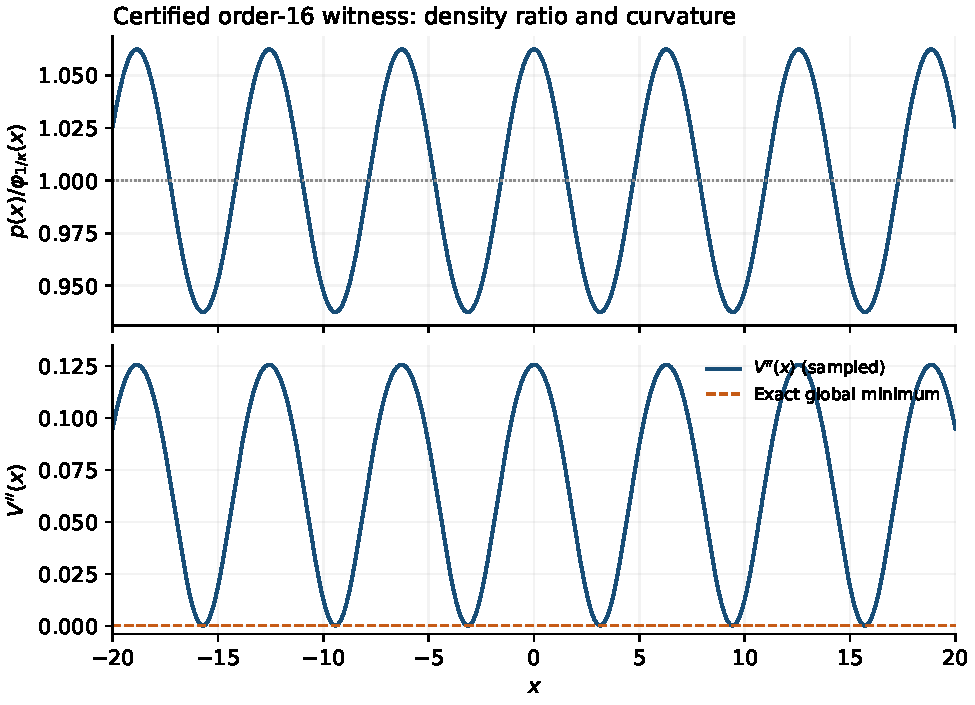
\includegraphics[width=.9\textwidth]{witness16.pdf}
\caption{The explicit order-16 density relative to its Gaussian envelope, and
its potential curvature. The plot is illustrative; the global lower bound
and negative entropy derivative are established by the certificates.}
\end{figure}

\begin{table}[htbp]
\centering
\begin{tabular}{rrc}
\toprule
$m$ & Approximate $S_m(p)$ & Certified sign \\
\midrule
6 & $0.0047085551$ & positive \\
7 & $0.0081424992$ & positive \\
8 & $0.014996902$ & positive \\
12 & $0.28116197$ & positive \\
13 & $0.61425205$ & positive \\
14 & $1.248398$ & positive \\
15 & $1.8940176$ & positive \\
16 & $-0.57212968$ & negative \\
17 & $-14.928482$ & negative \\
18 & $93.05105$ & positive \\
19 & $3571.2182$ & positive \\
20 & $60128.674$ & positive \\
\bottomrule
\end{tabular}
\caption{Derivatives of the same explicit order-16 witness. Displayed values are rounded midpoints; signs are rigorously certified. Full enclosures are in \texttt{certs/witness\_order\_table/}. These are statements about this density only.}
\end{table}

